\documentclass[journal=esthag,manuscript=suppinfo]{achemso}

% additional packages
\usepackage[utf8]{inputenc}
\usepackage{amsmath}
\usepackage{booktabs}
\usepackage{subcaption}
\usepackage{array,multirow,graphicx}
\graphicspath{{./../figures/}}
% macros

% authors
\author{Jonathan G. V. Ström}
\affiliation[Brown University]{Brown University, School of Engineering, Providence, RI, USA}
\author{Yuanming Guo}
\affiliation[Arizona State University]{Arizona State University, School of Sustainable Engineering and the Building Environment, Tempe, AZ, USA}
\author{Yijun Yao}
\affiliation[Brown University]{Brown University, School of Engineering, Providence, RI, USA}
\author{Eric M. Suuberg}
\email{eric_suuberg@brown.edu}
\affiliation[Brown University]{Brown University, School of Engineering, Providence, RI, USA}

% title
\title{Temporal Variations In Vapor Intrusion-Induced Indoor Air Contaminant Concentrations}

% keywords
\abbreviations{VI}
\keywords{Vapor intrusion, Preferential pathways, Temporal variability, Finite element modeling, Air exchange rate, Indoor/outdoor pressure difference}

\begin{document}

\newpage
\subsection{Pressure and Air Exchange Rate}
\begin{figure}
  \caption{2D KDE figure showing distributions and relationship between indoor/outdoor pressure difference and air exchange rate. The seasonal median $p_\mathrm{in/out}$ and $A_e$ are indicated by the location of the respective arrow tips. Only non-CPM period considered.}
  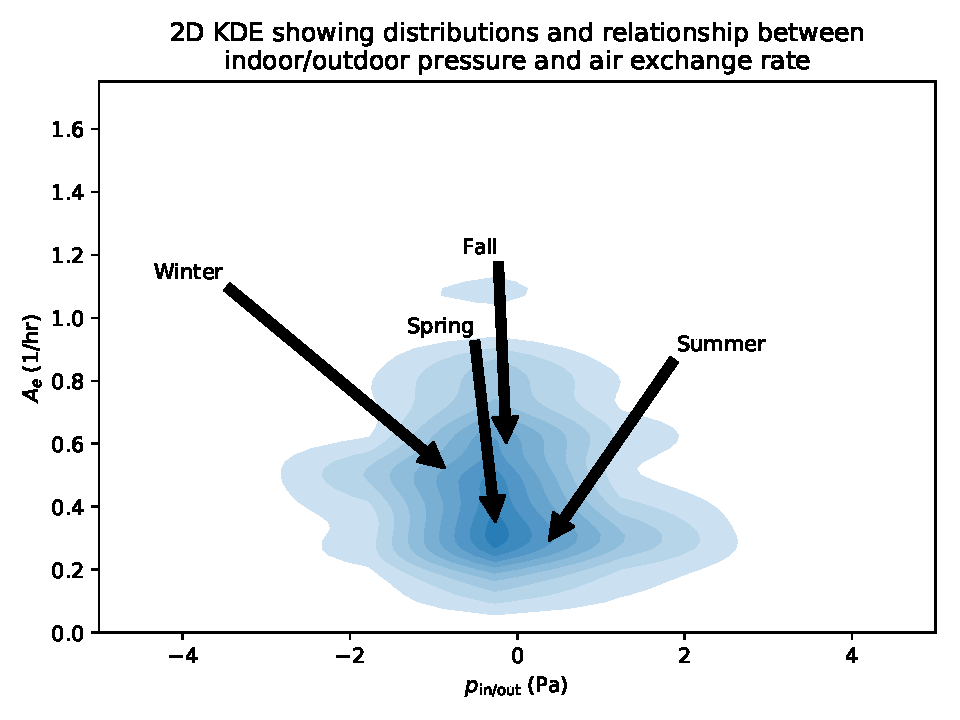
\includegraphics[width=\textwidth]{pressure_air_exchange_rate.pdf}
\end{figure}

\end{document}
